\documentclass[aspectratio=169]{beamer}

% The  following themes, you can uncomment it to use
% Want to figure out  what theme you have  on your computer(this refers to linux distro) that you can use
% the following cpmmand may help you:
%
% ls /usr/share/texlive/texmf-dist/tex/latex/beamer | grep "^beamertheme"
%
% Or you can go to:
% https://deic.uab.cat/~iblanes/beamer_gallery/   to see more info

%%%%%%%%%%%%%%%%%%%%%%%%%%%%%%%%%%%%%%%%
% \usetheme[named=mygreen]{Berkeley}
% \usetheme{Warsaw}
 \usetheme{metropolis} % reference:https://mirror.mwt.me/ctan/macros/latex/contrib/beamer-contrib/themes/metropolis/doc/metropolistheme.pdf
% \usetheme{AnnArbor}
% \usetheme{Berlin}
% \usecolortheme{crane}
% \usecolortheme{seahorse}
% \usecolortheme{dolphin}
%%%%%%%%%%%%%%%%%%%%%%%%%%%%%%%%%%%%%%%%

%%%%%%%%%%%%%%%%%%%%%%%%%%%%%%%%%%%%%%%%
% support for chinese
%%%%%%%%%%%%%%%%%%%%%%%%%%%%%%%%%%%%%%%%
\usepackage{ctex}

%%%%%%%%%%%%%%%%%%%%%%%%%%%%%%%%%%%%%%%%
% support for images and set the image path
%%%%%%%%%%%%%%%%%%%%%%%%%%%%%%%%%%%%%%%%
\usepackage{graphicx}
\graphicspath{ {./images/} }


%%%%%%%%%%%%%%%%%%%%%%%%%%%%%%%%%%%%%%%%
% support for table
%%%%%%%%%%%%%%%%%%%%%%%%%%%%%%%%%%%%%%%%
\usepackage{multirow}

%    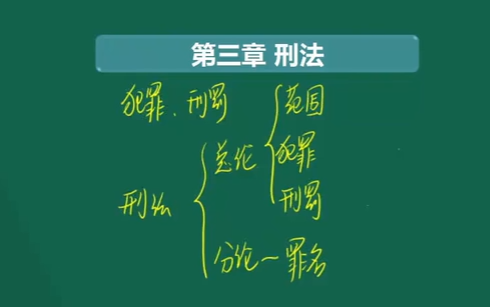
\includegraphics[scale=0.5]{criminal_law_intro}\\ 

%%%%%%%%%%%%%%%%%%%%%%%%%%%%%%%%%%%%%%%%
% support for basic color
%  
% \textcolor{red/blue/green/black/white/cyan/magenta/yellow}{text}
%  
%%%%%%%%%%%%%%%%%%%%%%%%%%%%%%%%%%%%%%%%
\usepackage{color}



\begin{document}
%
% Basic Information Of This Silde
%

\title{2019 年 6 月广东深圳市属事业单位招聘《行政职业能力测试》真题}
\author{aka}
\institute{aka}
\date{\today}

%%%%%%%%%%%%%%%%%%%%%%%%%%%%%%%%%%%%%%%%
% titlepage
%%%%%%%%%%%%%%%%%%%%%%%%%%%%%%%%%%%%%%%%
\begin{frame}
\titlepage
\end{frame}


%%%%%%%%%%%%%%%%%%%%%%%%%%%%%%%%%%%%%%%%
% A frame
%%%%%%%%%%%%%%%%%%%%%%%%%%%%%%%%%%%%%%%%
\begin{frame}[t]{数量关系}
    \textbf{1、}
    1,1,2,4,7,13,( )\\
    A、15\\
    B、19\\
    C、22\\
    D、24\\
\end{frame}

%%%%%%%%%%%%%%%%%%%%%%%%%%%%%%%%%%%%%%%%
% A frame
%%%%%%%%%%%%%%%%%%%%%%%%%%%%%%%%%%%%%%%%
\begin{frame}[t]{数量关系}
    \textbf{1、}
    1,1,2,4,7,13,( )\\
    A、15\\
    B、19\\
    C、22\\
    D、24\\
    解析:\textcolor{red}{D}\\
    数列无明显特征,多级作差无规律,考虑递推。观察发现:\\
    $1+1+2=4$,\\
    $1+2+4=7$,\\
    $2+4+7=13$,\\
    $4+7+13=24$\\
    即从第四项开始,每一项都等于前三项数字之和\\
\end{frame}


%%%%%%%%%%%%%%%%%%%%%%%%%%%%%%%%%%%%%%%%
% A frame
%%%%%%%%%%%%%%%%%%%%%%%%%%%%%%%%%%%%%%%%
\begin{frame}[t]{数量关系}
    \textbf{2、}-2,-4,0,16,( )
    A、20\\
    B、30\\
    C、40\\
    D、50\\
\end{frame}


%%%%%%%%%%%%%%%%%%%%%%%%%%%%%%%%%%%%%%%%
% A frame
%%%%%%%%%%%%%%%%%%%%%%%%%%%%%%%%%%%%%%%%
\begin{frame}[t]{数量关系}
    \textbf{2、} $-2$,$-4$,0,16,( )\\
    A、20\\
    B、30\\
    C、40\\
    D、50\\
    解析:\textcolor{red}{D}\\
    2、数列无明显特征,多级与递推均无规律,且大部分数为合数,考虑因数分解。原数列可分别分解为:\\
    $-2 \times 1^2$\\
    $-1 \times 2^2$\\
    $0 \times 3^2$\\
    $1 \times 4^2$\\
    $2 \times 5^2$\\
\end{frame}



%%%%%%%%%%%%%%%%%%%%%%%%%%%%%%%%%%%%%%%%
% A frame
%%%%%%%%%%%%%%%%%%%%%%%%%%%%%%%%%%%%%%%%
\begin{frame}[t]{数量关系}
    \textbf{3、}1,1,4,8,9,27,16,( )\\
    A、63\\
    B、64\\
    C、25\\
    D、26\\
\end{frame}


%%%%%%%%%%%%%%%%%%%%%%%%%%%%%%%%%%%%%%%%
% A frame
%%%%%%%%%%%%%%%%%%%%%%%%%%%%%%%%%%%%%%%%
\begin{frame}[t]{数量关系}
    \textbf{3、}1,1,4,8,9,27,16,( )\\
    A、63\\
    B、64\\
    C、25\\
    D、26\\
    解析:\textcolor{red}{B}\\
    数列项数较多,优先考虑多重数列。\\
    奇数项构成平方数列,可以表示为:\\
    $1^2, 2^2, 3^2, 4^2$\\
    偶数项构成立方数列,可以表示为:\\
    $1^3, 2^3, 3^3$\\
    底数是公差为 1 的等差数列, 所求项$=(3+1)^3 = 64$\\
\end{frame}


%%%%%%%%%%%%%%%%%%%%%%%%%%%%%%%%%%%%%%%%
% A frame
%%%%%%%%%%%%%%%%%%%%%%%%%%%%%%%%%%%%%%%%
\begin{frame}[t]{数量关系}
    \textbf{4、}5,11,24,52,( )\\
    A、88 \\
    B、112\\
    C、130\\
    D、156\\
\end{frame}

%%%%%%%%%%%%%%%%%%%%%%%%%%%%%%%%%%%%%%%%
% A frame
%%%%%%%%%%%%%%%%%%%%%%%%%%%%%%%%%%%%%%%%
\begin{frame}[t]{数量关系}
    \textbf{4、}5,11,24,52,( )\\
    A、88 \\
    B、112\\
    C、130\\
    D、156\\
    解析:\textcolor{red}{B}\\
    数列无明显特征,多级无规律,考虑递推。观察发现:\\
    $2 \times 5 = 10, 10+1=11$\\
    $2 \times 11 = 22, 22+2=24$\\
    $2 \times 24 = 48, 48+4=52$\\
    $2 \times 52 = 104, 104+8=112$\\
\end{frame}


%%%%%%%%%%%%%%%%%%%%%%%%%%%%%%%%%%%%%%%%
% A frame
%%%%%%%%%%%%%%%%%%%%%%%%%%%%%%%%%%%%%%%%
\begin{frame}[t]{数量关系}
    \textbf{5、}8,24,16,20,18,( )\\
    A、19\\
    B、20\\
    C、21\\
    D、22\\
\end{frame}

%%%%%%%%%%%%%%%%%%%%%%%%%%%%%%%%%%%%%%%%
% A frame
%%%%%%%%%%%%%%%%%%%%%%%%%%%%%%%%%%%%%%%%
\begin{frame}[t]{数量关系}
    \textbf{5、}8,24,16,20,18,( )\\
    A、19\\
    B、20\\
    C、21\\
    D、22\\
    解析:\textcolor{red}{A}\\
    方法一:数列无明显特征,考虑多级作差。后项减前项,得到新数列:\\
    $16, -8, 4, -2, 1$,构成公比为 $-\frac{1}{2}$的等比数列, 故所求项为$18+1=19$\\
    方 法 二 : 观 察可得: \\
    $(8+24) \div 2 = 16$\\
    $(24+16) \div 2 = 20$\\
    $(20+18) \div 2 = 19$\\
\end{frame}


%%%%%%%%%%%%%%%%%%%%%%%%%%%%%%%%%%%%%%%%
% A frame
%%%%%%%%%%%%%%%%%%%%%%%%%%%%%%%%%%%%%%%%
\begin{frame}[t]{数量关系}
    6、甲,乙两站均为每隔 50 分钟同时对向发一趟客车,客车从甲站到乙站,单程需行驶 4 小时,每辆客车
的行驶速度相同,某旅客乘车从甲站到乙站,他在行程中最多可以遇到从乙站开往甲站的客车( )辆\\
A、10\\
B、9\\
C、8\\
D、5\\
\end{frame}


%%%%%%%%%%%%%%%%%%%%%%%%%%%%%%%%%%%%%%%%
% A frame
%%%%%%%%%%%%%%%%%%%%%%%%%%%%%%%%%%%%%%%%
\begin{frame}[t]{数量关系}
    6、甲,乙两站均为每隔 50 分钟同时对向发一趟客车,客车从甲站到乙站,单程需行驶 4 小时,每辆客车
的行驶速度相同,某旅客乘车从甲站到乙站,他在行程中最多可以遇到从乙站开往甲站的客车( )辆\\
A、10\\
B、9\\
C、8\\
D、5\\
    解析:\textcolor{red}{B},
    单程 4 小时, 即 $4 \times 60 = 240min$ ,
    由于甲乙同时发车, 旅客会遇到在他启程前已经从乙车站出发还没到达的汽车和启程后在乙车站出发的汽车,
    由于每 50 分钟 出发一辆,$240=50+50+50+50+40$ 之前出发未到的车中有一辆还差 40 分钟到达,
    由于速度相同,则乘客出发后 20 分钟可遇到第一辆车,此时还剩下$240-20=220 min$,因为两个车同时走,所以接下的时间每 $(50 \div 2) = 25 min$ 遇到一辆车,
    则$(220 \div 5 ) = 8...20$ 则遇到 8 辆车, 总共遇到 $8+1=9$ 辆车。

\end{frame}



%%%%%%%%%%%%%%%%%%%%%%%%%%%%%%%%%%%%%%%%
% A frame
%%%%%%%%%%%%%%%%%%%%%%%%%%%%%%%%%%%%%%%%
\begin{frame}[t]{数量关系}
    7、某人 2012 的年龄是 3 的倍数,2013 年的年龄是 4 的倍数,2014 年的年龄是 5 的倍数,则此人 2015 年
的年龄是( )岁。\\
A、56\\
B、60\\
C、61\\
D、66\\
    解析:\textcolor{red}{D}\\
    A.2015 年 56 岁,则 2012 年为 $56-3 = 53$,不是 3 的倍数,排除;\\
    B.2015 年 60 岁,则 2012 年为 $60-3 = 57$,是 3 的倍数,2013 年为 $57+1 = 58$,不是 4 的倍数\\
    C.2015 年 61 岁,则 2012 年为 $61-3 = 58$,不是 3 的倍数,排除;\\
    D.2015 年 66 岁,则 2012 年为 $66-3 = 63$,是 3 的倍数,2013 年为 $63+1 = 64$,是 4 的倍数,2014
年为 $63+2 = 65$,是 5 的倍数,正确。\\
\end{frame}



%%%%%%%%%%%%%%%%%%%%%%%%%%%%%%%%%%%%%%%%
% A frame
%%%%%%%%%%%%%%%%%%%%%%%%%%%%%%%%%%%%%%%%
\begin{frame}[t]{数量关系}
8、有十名高级工匠的工号依次为 1——10,若从中调走一名,则其余 9 名的工号的平均值较原来减少了 0.5,
调走的高级工证的工号是( )。\\
A、3\\
B、7\\
C、8\\
D、10\\
\end{frame}



%%%%%%%%%%%%%%%%%%%%%%%%%%%%%%%%%%%%%%%%
% A frame
%%%%%%%%%%%%%%%%%%%%%%%%%%%%%%%%%%%%%%%%
\begin{frame}[t]{数量关系}
8、有十名高级工匠的工号依次为 1——10,若从中调走一名,则其余 9 名的工号的平均值较原来减少了 0.5,
调走的高级工证的工号是( )。\\
A、3\\
B、7\\
C、8\\
D、10\\
    解析:\textcolor{red}{D}\\
    调走前平均值$\frac{(1+2+3+4+5+6+7+8+9+10)}{10} = \frac{55}{10} = 5.5$\\
    调走后平均值$5.5 - 0.5 = 5$, 调走后还剩 9 人,则$(5\times9) = 45$\\
    则调走的人的工号为 $55-45=10$\\
\end{frame}


%%%%%%%%%%%%%%%%%%%%%%%%%%%%%%%%%%%%%%%%
% A frame
%%%%%%%%%%%%%%%%%%%%%%%%%%%%%%%%%%%%%%%%
\begin{frame}[t]{数量关系}
    9、某研究生院今年的研一新生共 1305 人,比去年增加了 4.4\%,其中女生人数减少 4\%,男生人数增加 10\%,
则该院今年的研一新生中有男生( )人。\\
A、790\\
B、805\\
C、825\\
D、865\\
\end{frame}


%%%%%%%%%%%%%%%%%%%%%%%%%%%%%%%%%%%%%%%%
% A frame
%%%%%%%%%%%%%%%%%%%%%%%%%%%%%%%%%%%%%%%%
\begin{frame}[t]{数量关系}
    9、某研究生院今年的研一新生共 1305 人,比去年增加了 4.4\%,其中女生人数减少 4\%,男生人数增加 10\%,
则该院今年的研一新生中有男生( )人。\\
A、790\\
B、805\\
C、825\\
D、865\\
    解析:\textcolor{red}{C}\\
    今年的研一新生共 1305 人,比去年增加了4.4\% ,则去年研一新生总人数$=\frac{1035}{1+4.4\%}= 1250$ \\
    根据线段法,女生与男生人数的增长率的线段距离之比为$\frac{4.4\%-(-4\%)}{10\% - 4.4\%} = \frac{8.4\%}{5.6\%} = \frac{3}{2}$\\
    ,由于增长率线段距离之比与基期量成反比,则有去年女生与男生的人数之比为 2:3,因此去年男生的人数为 $\frac{1250}{2+3} \times 3 = 750$,
    则今年的研一新生中男生人数为 $750 \times (1+10\%) = 825$ \\
\end{frame}

%%%%%%%%%%%%%%%%%%%%%%%%%%%%%%%%%%%%%%%%
% A frame
%%%%%%%%%%%%%%%%%%%%%%%%%%%%%%%%%%%%%%%%
\begin{frame}[t]{数量关系}
    9、某研究生院今年的研一新生共 1305 人,比去年增加了 4.4\%,其中女生人数减少 4\%,男生人数增加 10\%,
则该院今年的研一新生中有男生( )人。\\
A、790\\
B、805\\
C、825\\
D、865\\
    解析:\textcolor{red}{C}\\
    方法二: 今年的研一新生男生数 = 去年男生数 $\times (1+10\%)  = 1.1 \times $ 去年男生数,即 
    今年男生人数/去年男生人数 $= \frac{11}{10}$ \\
人数必须为整数,所以今年男生人数必须为 11 的倍数,仅 C 项符合。\\
\end{frame}




%%%%%%%%%%%%%%%%%%%%%%%%%%%%%%%%%%%%%%%%
% A frame
%%%%%%%%%%%%%%%%%%%%%%%%%%%%%%%%%%%%%%%%
\begin{frame}[t]{数量关系}
    10、某项目由甲乙二人竞标,以所报单价高者胜,甲从 10 元,11 元,12 元,13 元,16 元,17 元六个单
价中随机选择一个作为合作价,乙从 13 元,14 元,15 元中随机选取一个作为报价,则乙中标的概率为( )。\\
    A、$\frac{7}{18}$  \\
    B、$\frac{11}{18}$ \\
    C、$\frac{2}{3} $  \\
    D、$\frac{5}{6} $  \\
\end{frame}


%%%%%%%%%%%%%%%%%%%%%%%%%%%%%%%%%%%%%%%%
% A frame
%%%%%%%%%%%%%%%%%%%%%%%%%%%%%%%%%%%%%%%%
\begin{frame}[t]{数量关系}
    10、某项目由甲乙二人竞标,以所报单价高者胜,甲从 10 元,11 元,12 元,13 元,16 元,17 元六个单
价中随机选择一个作为合作价,乙从 13 元,14 元,15 元中随机选取一个作为报价,则乙中标的概率为( )。\\
    A、$\frac{7}{18}$  \\
    B、$\frac{11}{18}$ \\
    C、$\frac{2}{3} $  \\
    D、$\frac{5}{6} $  \\
    解析:\textcolor{red}{C}\\
    根据概率公式 $p=$ 满足总情况数/总数, 甲有 6 种报价方式,乙有 3 种报价方式,则总数为 种,满足
条件的情况数有以下几种\\
乙报价为 13 元,甲报价为 10 元,11 元,12 元时,乙可以中标,共 3 种情况;\\
乙报价为 14 元,甲报价为 10 元,11 元,12 元,13 元时,乙可以中标,共 4 种情况;\\
乙报价为 15 元,甲报价为 10 元,11 元,12 元,13 元时,乙可以中标,共 4 种情况\\
    因此乙能中标的情况为 $3+4+4 = 11$ 种, 则 概率 $p=\frac{11}[18]$\\

\end{frame}



%%%%%%%%%%%%%%%%%%%%%%%%%%%%%%%%%%%%%%%%
% A frame
%%%%%%%%%%%%%%%%%%%%%%%%%%%%%%%%%%%%%%%%
\begin{frame}[t]{言语理解}
    11、仅仅把环境保护理解为人“聪明的自利”,尊重和维护自然的全部目的也仅仅是为了人的利
    益,这样的思想也()有些狭隘了\\
A、不免\\
B、未免\\
C、难免\\
D、以免\\
\end{frame}

%%%%%%%%%%%%%%%%%%%%%%%%%%%%%%%%%%%%%%%%
% A frame
%%%%%%%%%%%%%%%%%%%%%%%%%%%%%%%%%%%%%%%%
\begin{frame}[t]{言语理解}
    11、仅仅把环境保护理解为人“聪明的自利”,尊重和维护自然的全部目的也仅仅是为了人的利
    益,这样的思想也()有些狭隘了\\
A、不免 \qquad B、未免\\
C、难免 \qquad  D、以免\\
    解析:\textcolor{red}{B}\\
“这样的思想”指代的是前文“仅仅把环境保护……,尊重和维护自然的全部目的也仅仅是……”,
由“仅仅”可知,这样的思想确实片面、狭隘,故横线处应对前文观点予以否定,B 项,“未免”意为实在是,
不能不说是,多指人对过分的事情不以为然,或委婉给予否定的评价,符合文意,当选。
A 项,“不免”意为避免不了或难以避免,并非对前文观点语义否定,排除。
C 项,“难免”强调的是某种结果不容易避免,多用于规律性情况或有一种解释或宽慰的语气,暗含没什
么,事情不严重之意,文中并未有思想狭隘不严重之意,排除。
D 项,“以免”多用于提起下半句话,表明前半句话是为了使下半句话所说的情形不至于发生,填入后与
文意相悖,排除。
\end{frame}


%%%%%%%%%%%%%%%%%%%%%%%%%%%%%%%%%%%%%%%%
% A frame
%%%%%%%%%%%%%%%%%%%%%%%%%%%%%%%%%%%%%%%%
\begin{frame}[t]{言语理解}
    12、将下列选项中的词语依次填入各句横线处,最恰当的一组是:\\
    (1)生活中的长久沉积,犹如陈年佳酿,其味越来越()、绵长。\\
   (2)只见他神情自若地从口袋里掏出窃来的讲稿,对着在座的教授们口若悬河、()地讲开了。\\
\textbf{A}醇正,振振有词
\textbf{B}醇正,念念有词
\textbf{C}纯正,振振有词
\textbf{D}纯正,念念有词\\
 解析:\textcolor{red}{A}
    第(1)句,横线处用  来形容陈年佳酿的味道,A、B 项的“醇正”指酒的品质厚重柔和,不仅正宗绵
甜,而且回味悠长,可与“陈年佳酿”搭配,保留。C、D 项的“纯正”指纯粹;不搀杂其他成分,多与“性情、
品格”等搭配,用于此处不当,排除;
第(2)句,横线处需与“口若悬河”构成并列,且对应前文的“窃来的讲稿”,故横线处应填入表示不停
说话或说很多的贬义词,A 项“振振有词”意为理直气壮的样子。借以形容自以为理由充分,说个没完。多用
作贬义。符合文意,当选。B 项“念念有词”旧指迷信的人祈祷时不停地念着口语,以通神灵,现多用来形容
人嘟嘟囔囔说个不停。填入横线处感情色彩不如 A 项恰当,对比择优,排除
\end{frame}



%%%%%%%%%%%%%%%%%%%%%%%%%%%%%%%%%%%%%%%%
% A frame
%%%%%%%%%%%%%%%%%%%%%%%%%%%%%%%%%%%%%%%%
\begin{frame}[t]{言语理解}
    13、将下列选项中的词语依次填入各句横线处,最恰当的一组是:\\
    (1)精灵鬼怪,花草树木,宫殿楼阁都在这个()的世界里被安徒生的妙笔赋予了生命。\\
    (2)从前研究中国文化的人,往往只看高层次的思想,意识形态,而忽视了现实生活中很多和观念文化理
    想冲突的方面,这样的文化研究者,就是犯了()的错误。\\
    A、光怪陆离,目无全牛\\
    B、光怪陆离,以偏概全\\
    C、斑驳陆离,目无全牛\\
    D、斑驳陆离,以偏概全\\
\end{frame}



%%%%%%%%%%%%%%%%%%%%%%%%%%%%%%%%%%%%%%%%
% A frame
%%%%%%%%%%%%%%%%%%%%%%%%%%%%%%%%%%%%%%%%
\begin{frame}[t]{言语理解}
 解析:\textcolor{red}{B}\\
    第一空,修饰“安徒生的童话世界”,“光怪陆离”形容事物离奇多变,奇形怪状、五颜六色,对应
前文“精灵鬼怪,花草树木,宫殿楼阁”,体现出安徒生的童话世界多样精彩,A、B 两项保留;\\
    “斑驳陆离”
形容颜色繁杂、斑驳绚丽,不能与童话世界搭配,排除 C、D 两项。\\

第二空,搭配“错误”,感情色彩消极,B 项“以偏概全”指用片面的观点看待整体问题,感情色彩消极,
符合文意,当选;\\
    A 项“目无全牛”比喻技术熟练到了得心应手的境地,感情色彩积极褒义,排除。
故正确答案为 B
\end{frame}



%%%%%%%%%%%%%%%%%%%%%%%%%%%%%%%%%%%%%%%%
% A frame
%%%%%%%%%%%%%%%%%%%%%%%%%%%%%%%%%%%%%%%%
\begin{frame}[t]{言语理解}
14、将下列选项中的词语依次填入句子横线处,最恰当的一组是:\\
    在小数据时代,人们可以通过数据和分析来验证猜想,以上世纪 80 年代文学为例,文学()能成为
    社会热点。与文学生产相对有限且思想表现集中在思想启蒙上有直接关系,()与出版流通相对缓慢有关。\\
    如研究改革文学,彼时的文学批评者完全可以穷尽有限的文本。()遗漏一些文本,批评家()可
以言之凿凿,所作的推论基本有效。\\
A、一方面,另一方面,尽管,还是\\
B、一方面,另一方面,如果,就\\
C、之所以,还,即便,仍然\\
D、之所以,还,只要,就\\
\end{frame}


%%%%%%%%%%%%%%%%%%%%%%%%%%%%%%%%%%%%%%%%
% A frame
%%%%%%%%%%%%%%%%%%%%%%%%%%%%%%%%%%%%%%%%
\begin{frame}[t]{言语理解}
    解析:\textcolor{red}{C}\\
    14、根据“在思想启蒙上有直接关系”可知,“出版流通相对缓慢有关”是文学能成为社会热点的第二个
原因,故前两空之间应该填入因果关系的关联词,对应 C、D 项保留;\\
    “一方面……另一方面”为并列关系,排除 A、B 两项。\\
    第二空,前文“遗漏文本”,后文批评家的推论还是能够有效,说明两句话之间存在假设关系,
即便遗漏一些文本,仍然可以言之凿凿,推论基本有效,对应 C 项,当选;D 项“只要……就”为条件关系,
不符合文段逻辑,排除。
故正确答案为 C
\end{frame}



%%%%%%%%%%%%%%%%%%%%%%%%%%%%%%%%%%%%%%%%
% A frame
%%%%%%%%%%%%%%%%%%%%%%%%%%%%%%%%%%%%%%%%
\begin{frame}[t]{言语理解}
15、将下列选项中的词语依次填入各句横线处,最恰当的一组是:\\
    (1)如今,企业经营者们都多了一些理性的思考和判断,盲目炒卖房地产的现象有所缓解。而() 的房地产公司已自消自灭,一些无经营实力,想玩“空手道”的公司也难以得手。\\
(2)他用行动证明了只要肯付诸行动,不怕90,而且有毅力坚持下去,天底下就没有战不胜的困
难。\\
A、出风头,碰钉子\\
B、出风头,敲竹杠\\
C、赶浪头,敲竹杠\\
D、赶浪头,碰钉子\\
\end{frame}

%%%%%%%%%%%%%%%%%%%%%%%%%%%%%%%%%%%%%%%%
% A frame
%%%%%%%%%%%%%%%%%%%%%%%%%%%%%%%%%%%%%%%%
\begin{frame}[t]{言语理解}
    解析:\textcolor{red}{D}\\
    15、第一空,根据“盲目炒卖房地产的现象有所缓解”可知,横线处填入词语应体现出房地产公司借机敛
财之意,“赶浪头”指比喻紧紧追随时尚,做适应当前形势的事,符合文意。“出风头”指出头露面显示自己,
与文意无关,故排除 A、B 两项。\\
第二空,根据“天底下就没有战不胜的困难”可知,横线处词语应体现出困难之意,D 项“碰钉子”比喻
遭到拒绝或受到斥责,有遇到困难的意思。C 项“敲竹杠”指利用别人的弱点或借某种口实抬高价格或索取财
物,与文意无关,排除。\\
故正确答案为 D\\
\end{frame}



%%%%%%%%%%%%%%%%%%%%%%%%%%%%%%%%%%%%%%%%
% A frame
%%%%%%%%%%%%%%%%%%%%%%%%%%%%%%%%%%%%%%%%
\begin{frame}[t]{言语理解}
16、下列各句中,没有语病的是( )。\\
A、历代古今中外的经验证明,教育孩子要重视榜样的作用,特别是家长的榜样作用。\\
B、经过市立学院几位专家的指导,让该市葡萄的产量和质量都得到了很大的改善。\\
C、有少数观众素质不高,当参赛选手出现因过度紧张而未正常发挥技术或有所失误时,便嘘声四起。\\
D、据统计,“好读书”基金在过去的十余年里,一共积累了逾千万元的助学奖金。\\
\end{frame}

%%%%%%%%%%%%%%%%%%%%%%%%%%%%%%%%%%%%%%%%
% A frame
%%%%%%%%%%%%%%%%%%%%%%%%%%%%%%%%%%%%%%%%
\begin{frame}[t]{言语理解}
    解析:\textcolor{red}{D}\\
    16、A 项,“历代”赘余,因“古今中外”即含有“历代”的意思,排除;\\
    B 项,“经过……让”缺少主语,成分残缺,排除;\\
    C 项,语序不当,“因过度紧张而”作为状语,应在“出现”之前,且“出现”与“未正常发挥技术”不
    能搭配使用,应为“出现未正常发挥技术的情况”,排除;\\
    D 项,表述正确,当选。\\
    故正确答案为 D\\
\end{frame}




%%%%%%%%%%%%%%%%%%%%%%%%%%%%%%%%%%%%%%%%
% A frame
%%%%%%%%%%%%%%%%%%%%%%%%%%%%%%%%%%%%%%%%
\begin{frame}[t]{言语理解}
17、下列各句中,有语病的是( )。\\
A、我国的经济发展仍处于可以大有作为的重要战略机遇期,蕴藏着巨大的潜力。\\
B、过去七年中,无良的汽车厂家在大约 1100 万辆柴油汽车上安装作弊软件以通过尾气排放检测。\\
C、虽然十分疲惫,但一想起几个月来一连串发生的怪事,那个老农民怎么也睡不着了。\\
D、“十三五”期间,生育政策作为备受关注的一项公共政策,其可能发生的变化值得各方期待。\\
\end{frame}



%%%%%%%%%%%%%%%%%%%%%%%%%%%%%%%%%%%%%%%%
% A frame
%%%%%%%%%%%%%%%%%%%%%%%%%%%%%%%%%%%%%%%%
\begin{frame}[t]{言语理解}
    17、下列各句中,有语病的是( )。\\
    A、我国的经济发展仍处于可以大有作为的重要战略机遇期,蕴藏着巨大的潜力。\\
    B、过去七年中,无良的汽车厂家在大约 1100 万辆柴油汽车上安装作弊软件以通过尾气排放检测。\\
    C、虽然十分疲惫,但一想起几个月来一连串发生的怪事,那个老农民怎么也睡不着了。\\
    D、“十三五”期间,生育政策作为备受关注的一项公共政策,其可能发生的变化值得各方期待。\\

    解析:\textcolor{red}{C}\\
    C 项,定语误放在状语位置,应改为“发生的一连串怪事”,故语序不当,当选;\\
    A 项、B 项、D 项,均表述正确,排除。\\
    本题为选非题,故正确答案为 C\\
\end{frame}



%%%%%%%%%%%%%%%%%%%%%%%%%%%%%%%%%%%%%%%%
% A frame
%%%%%%%%%%%%%%%%%%%%%%%%%%%%%%%%%%%%%%%%
\begin{frame}[t]{言语理解}
18、说到这个问题,他从资料箱里拿出十几封信,其中一封来自 S 区保安大队全体保安写的。以上句子所
属的语病类型是( )。\\
A、成分残缺\\
B、句式杂糅\\
C、语序不当\\
D、搭配不当 \\
\end{frame}


%%%%%%%%%%%%%%%%%%%%%%%%%%%%%%%%%%%%%%%%
% A frame
%%%%%%%%%%%%%%%%%%%%%%%%%%%%%%%%%%%%%%%%
\begin{frame}[t]{言语理解}
18、说到这个问题,他从资料箱里拿出十几封信,其中一封来自 S 区保安大队全体保安写的。以上句子所
属的语病类型是( )。\\
A、成分残缺\\
B、句式杂糅\\
C、语序不当\\
D、搭配不当 \\
    解析:\textcolor{red}{B}\\
    文中语句可以说“说到这个问题,他从资料箱里拿出十几封信,其中一封来自 S 区保安大队全体保安”,
也可以说“说到这个问题,他从资料箱里拿出十几封信,其中一封是 S 区保安大队全体保安写的”,故本句属
于句式杂糅的错误。\\
故正确答案为 B\\
\end{frame}




%%%%%%%%%%%%%%%%%%%%%%%%%%%%%%%%%%%%%%%%
% A frame
%%%%%%%%%%%%%%%%%%%%%%%%%%%%%%%%%%%%%%%%
\begin{frame}[t]{言语理解}
19、下列各句中,有语病的是( )。\\
A、这是一座跨越了一千五百年的老建筑,在这里,哥特式风格与伊斯兰风格完美融合,营造出西班牙所特
有的人文环境。\\
B、未成年人保护观念的进步使得赖宁精神逐渐被淡化,但谁又能否认现在依然需要学习赖宁呢?\\
C、国际移民组织已启动一项旨在从几个方面帮助战后伊拉克重建的人道主义援助计划。\\
D、蛞蝓是一种高蛋白、低脂肪、营养丰富的软体动物,肉味光滑、白润,含有多种氨基酸、酶类和维生素,\\
还具有一定的药用功效。\\
\end{frame}


%%%%%%%%%%%%%%%%%%%%%%%%%%%%%%%%%%%%%%%%
% A frame
%%%%%%%%%%%%%%%%%%%%%%%%%%%%%%%%%%%%%%%%
\begin{frame}[t]{言语理解}
19、下列各句中,有语病的是( )。\\
A、这是一座跨越了一千五百年的老建筑,在这里,哥特式风格与伊斯兰风格完美融合,营造出西班牙所特
有的人文环境。\\
B、未成年人保护观念的进步使得赖宁精神逐渐被淡化,但谁又能否认现在依然需要学习赖宁呢?\\
C、国际移民组织已启动一项旨在从几个方面帮助战后伊拉克重建的人道主义援助计划。\\
D、蛞蝓是一种高蛋白、低脂肪、营养丰富的软体动物,肉味光滑、白润,含有多种氨基酸、酶类和维生素,\\
还具有一定的药用功效。\\
    解析:\textcolor{red}{B}\\
    D 项“肉味”与“光滑、白润”搭配不当,可改为“肉味鲜美”。\\
故正确答案为 D。\\
\end{frame}




%%%%%%%%%%%%%%%%%%%%%%%%%%%%%%%%%%%%%%%%
% A frame
%%%%%%%%%%%%%%%%%%%%%%%%%%%%%%%%%%%%%%%%
\begin{frame}[t]{言语理解}
20、把下面几个句子组成语意连贯的一段文字,排序正确的一项是( )。\\
(1)由于画院画家的风格过于近似。\\
(2)甚至假定越精彩、越优秀的画作越有可能出自徽宗皇帝之手也未必准确\\
(3)徽宗每创作一副精品,画院画家们便争相模仿\\
(4)尽管有过不少尝试,但事实上很难将他们的作品区分开来\\
(5)如果他们足够幸运,皇帝就会在他们画作上题签以示确认\\
A、3-5-1-4-2\\
B、3-5-4-2-1\\
C、1-4-2-3-5\\
D、1-3-5-4-2\\
\end{frame}



%%%%%%%%%%%%%%%%%%%%%%%%%%%%%%%%%%%%%%%%
% A frame
%%%%%%%%%%%%%%%%%%%%%%%%%%%%%%%%%%%%%%%%
\begin{frame}[t]{言语理解}
    解析:\textcolor{red}{A}\\
对比首句,1 句指出画院画家风格相似,3 句指出画院画家们便争相模仿徽宗的画作精品。对比两句发
现,应是画家们争相模仿一样的画作才导致他们风格相似,故 3 句应在 1 句之前,排除 C、D 项。\\
对比 A、B 项,判别 1 句与 4 句顺序,应是由于画家风格相似才产生画家的作品难以区别的结果,故 1 句应
在 4 句之前,排除 B 项,锁定 A 项。\\
故正确答案为 A
\end{frame}





%%%%%%%%%%%%%%%%%%%%%%%%%%%%%%%%%%%%%%%%
% A frame
%%%%%%%%%%%%%%%%%%%%%%%%%%%%%%%%%%%%%%%%
\begin{frame}[t]{言语理解}
21、溃疡病是一种常见的多因性疾病。在人体中一切器官都受到大脑管理,胃也包括其中。如果大脑皮层
受到某种有害刺激,其机能就会降低,比较低级的神经中枢的机能反而亢进,导致胃酸分泌增多,胃部肌肉紧
张性加强,供应胃血液的血管痉挛。由于一方面胃酸增加,一方面胃粘膜细胞血液供应不良,导致部分胃被消
化形成溃疡。长期溃疡病的疼痛刺激会影响并加重大脑皮层功能紊乱,进一步加重溃疡病,从而形成恶性循环。
临床实践中,因精神紧张、过度疲劳、恐惧忧伤等精神异常引起溃疡病发生且加重者屡见不鲜。如二战期间,
一些城市和军队溃疡病发生率明显升高,二战结束后,溃疡也迅速愈合了。\\
这段文字主要说明的是( )。\\
A、精神因素导致溃疡病产生的机制\\
B、二战期间溃疡病发生率升高的原因\\
C、胃溃疡产生的生理基础\\
D、精神健康是促使溃疡病痊愈的关键\\
\end{frame}


%%%%%%%%%%%%%%%%%%%%%%%%%%%%%%%%%%%%%%%%
% A frame
%%%%%%%%%%%%%%%%%%%%%%%%%%%%%%%%%%%%%%%%
\begin{frame}[t]{言语理解}
    解析:\textcolor{red}{A}\\
    文段开篇引出“溃疡病”这一话题,紧接着指出胃受到大脑管理,大脑皮层受刺激后,会导致溃疡病
产生甚至加重。并通过临床实践及二战期间的相关事例进行论证。故整个文段均在说明精神因素会导致溃疡病
的产生展开,对应 A 项。\\
B 项,“二战期间溃疡病发生率升高”对应后文举例说明的内容,非重点,排除;\\
C 项,“胃溃疡产生的生理基础”表述不明确,文段明确指出是精神因素导致溃疡病的产生,排除;\\
D 项,文段重点强调大脑皮层受到某种有害刺激,即精神紧张、大脑疲惫、恐惧忧伤等时会导致溃疡病产
生,并未明确指出溃疡病痊愈的关键,且“精神健康”仅对应“精神紧张”这一种刺激,表述片面,排除。\\
故正确答案为 A。\\
\end{frame}




%%%%%%%%%%%%%%%%%%%%%%%%%%%%%%%%%%%%%%%%
% A frame
%%%%%%%%%%%%%%%%%%%%%%%%%%%%%%%%%%%%%%%%
\begin{frame}[t]{言语理解}
22、行书的产生也是很早的,某种程度上可以说是与楷书、草书同时产生,因为所谓“行楷”“行草”,
只是很模糊的概念,没有绝对的界限。但是到了这三大书体各自成熟之后,彼此的风格与特点还是判然可分的。
无论如何,大概在魏晋时代,行书就开始在民间流行了。20 世纪初,我国新疆地区古楼兰国遗址出土了大量的
魏晋文书残纸,里头有不少已经是相当成熟的行书了。被称为“书圣”的东晋大书法家王羲之创作了大量的行
书作品,长期以来备受后人的珍爱。\\
下列说法与原文意思相符的是( )。\\
A、“行楷”“行草”没有绝对的界限,所以两者是同时产生的\\
B、成熟的行书、楷书和草书都是具有独特的风格与鲜明的特点\\
C、古楼兰国遗址出土的文书残纸说明在魏晋时行书已经普及\\
D、王羲之创作的行书属于相当成熟的行书作品,因此备受后人喜爱\\
\end{frame}



%%%%%%%%%%%%%%%%%%%%%%%%%%%%%%%%%%%%%%%%
% A frame
%%%%%%%%%%%%%%%%%%%%%%%%%%%%%%%%%%%%%%%%
\begin{frame}[t]{言语理解}
    解析:\textcolor{red}{B}\\
    、A 项,与文中“行书的产生也是很早的,某种程度上可以说是与楷书、草书同时产生,因为所谓“行
楷”“行草”,只是很模糊的概念,没有绝对的界限”对应,文段指出的是在某种程度上,行书与楷书、草书
同时产生,而并未提及“行楷”、“行草”产生的时间,与文意不符,排除;\\
B 项,对应文中“到了这三大书体各自成熟之后,彼此的风格与特点还是判然可分的”,表述正确,当选;\\
C 项,根据文中“我国新疆地区古楼兰国遗址出土了大量的魏晋文书残纸,里头有不少已经是相当成熟的
行书了”可知,出土的魏晋文书残纸仅能证明在魏晋时期行书比较成熟,而普及与否文段未提及,与文意不符,
排除;\\
D 项,与文中“被称为‘书圣’的东晋大书法家王羲之创作了大量的行书作品,长期以来备受后人的珍爱”
对应,文段未提及王羲之的行书备受后人喜爱的原因,与文意不符,排除。\\
故正确答案为 B。\\
\end{frame}





%%%%%%%%%%%%%%%%%%%%%%%%%%%%%%%%%%%%%%%%
% A frame
%%%%%%%%%%%%%%%%%%%%%%%%%%%%%%%%%%%%%%%%
\begin{frame}[t]{言语理解}
23、博物学家的幸福在某种程度上也依靠他的无知,无知给他留下这类新天地让他去征服。他可能在书本
上已经达到了知识的顶峰,但,在他用自己的眼睛证实每一个光辉的细节之前,他仍然感到是半无知的。
根据上文,下列对博物学家的分析正确的是( )。\\
A、博物学家因无知而能达到知识的顶峰\\
B、博物学家在一般人眼中其实也很无知\\
C、博物学家感到无知是因为所掌握的知识不切实际\\
D、博物学家因拥有新天地去征服而感到幸福\\
\end{frame}




%%%%%%%%%%%%%%%%%%%%%%%%%%%%%%%%%%%%%%%%
% A frame
%%%%%%%%%%%%%%%%%%%%%%%%%%%%%%%%%%%%%%%%
\begin{frame}[t]{言语理解}
    解析:\textcolor{red}{D}\\
    A 项,与文中“他可能在书本上已经达到了知识的顶峰”对应,文段并未说明无知与达到知识顶峰之
间存在因果关系,与文意不符,排除;\\
B 项,“博物学家在一般人眼中其实也很无知”,文段未提及,无中生有,排除;\\
C 项,与文中“在他用自己的眼睛证实每一个光辉的细节之前,他仍然感到是半无知的”对应,文段明确
指出,博物学家感到无知的原因是没有亲眼证实这些知识,并非掌握的知识不切实际,与文意不符,排除;\\
D 项,对应文中“博物学家的幸福在某种程度上也依靠他的无知,无知给他留下这类新天地让他去征服”,
表述正确,当选。\\
故正确答案为 D\\
\end{frame}




%%%%%%%%%%%%%%%%%%%%%%%%%%%%%%%%%%%%%%%%
% A frame
%%%%%%%%%%%%%%%%%%%%%%%%%%%%%%%%%%%%%%%%
\begin{frame}[t]{言语理解}
24、中国手工艺复兴是建立在传统文化复兴基础上的:喝茶、焚香、赏花、弹琴、作诗、论字画、把玩瓷
器、收藏古玩、穿中式衣服、摆中式家具,等等。这种生活方式已经在中国的白领阶层中形成新的时尚,也成
为了陶冶性情的一种方式。所谓,“器以载道”,正是这种新的时尚和新的陶冶性情的方式,为手工艺的复兴
打开了出路。而这些具有传统意味又有当代文人风尚的手工艺品的制作者,并非都是传统的手工艺人。其中包
括了那些从美院毕业的富有创造力的年轻艺术家们及设计师们,他们正在利用传统的手工技艺和传统的文化资
源创造新的中国时尚文化,这和民国时期梁漱溟“旧文化转变出一个新文化来”的理想何其相似。许多的传统
手工艺里还蕴含着“中国文化有形的根”而在这样的根底基础上创造出的器物文化与传统中国人“过日子的方
法”具有许多相通之处。\\
\end{frame}


%%%%%%%%%%%%%%%%%%%%%%%%%%%%%%%%%%%%%%%%
% A frame
%%%%%%%%%%%%%%%%%%%%%%%%%%%%%%%%%%%%%%%%
\begin{frame}[t]{言语理解}
下列说法与原文意思不符的是( )。\\
A、喝茶、焚香、赏花、弹琴、作诗、论字画等传统文化的复兴,为手工艺的复兴打开了出路\\
B、传统手艺人与美院毕业的艺术家,设计师都制作出了既有传统意味又有当代文人风尚的手工艺品\\
C、当代人通过利用传统的手工技艺和文化资源创造新的中国时尚文化,实现了梁漱溟“旧文化转变出个新
文化来”的理想\\
D、根植于中国文化的传统手工艺所创造出的器物文化,与传统中国人“过日子的方法”具有许多相通之处\\

\end{frame}



%%%%%%%%%%%%%%%%%%%%%%%%%%%%%%%%%%%%%%%%
% A frame
%%%%%%%%%%%%%%%%%%%%%%%%%%%%%%%%%%%%%%%%
\begin{frame}[t]{言语理解}
    解析:\textcolor{red}{C}\\
    A 项,对应文中“中国手工艺复兴是建立在传统文化复兴基础上的:喝茶、焚香、赏花、弹琴、作诗、
论字画、把玩瓷器、收藏古玩、穿中式衣服、摆中式家具,等等”,表述正确,排除;\\
B 项,根据文中“这些具有传统意味又有当代文人风尚的手工艺品的制作者,并非都是传统的手工艺人。
其中包括了那些从美院毕业的富有创造力的年轻艺术家们及设计师们”可知,选项表述正确,排除;\\
C 项,与文中“这和民国时期梁漱溟‘旧文化转变出一个新文化来’的理想何其相似”对应,文中说明当
代人创造新的中国时尚文化和梁漱溟的理想相似,而并非实现梁漱溟的理想,与文意不符,当选。\\
D 项,对应文中“许多的传统手工艺里还蕴含着‘中国文化有形的根’而在这样的根底基础上创造出的器
物文化与传统中国人“过日子的方法”具有许多相通之处”,表述正确,排除。\\
本题为选非题,故正确答案为 C\\
\end{frame}






%%%%%%%%%%%%%%%%%%%%%%%%%%%%%%%%%%%%%%%%
% A frame
%%%%%%%%%%%%%%%%%%%%%%%%%%%%%%%%%%%%%%%%
\begin{frame}[t]{言语理解}

25、果脯之所以会出现,是因为水果本身有季节性的特点,不耐保鲜,而果脯则一年四季都可以享用。在
不少人的心里,以为一般的果脯就是把鲜果晾晒制成的。其实果脯的制作是一个较为复杂的过程,需要经过脱
水等多项工艺的处理。虽然很多水果本身很甜,但是在加工过程中,为了保证口感,还会再加入大量的糖。如
此处理,水果中原本含有的水溶性维生素 C 大量流失,而热量超高的糖分却大大增加了。因此,果脯不能长期
过量食用,因为摄入过多的糖分,会导致人体中 B 族维生素和某些微量元素的缺乏。尤其是儿童,在饭前更不
宜食用果脯,否则还会影响食欲。另外,有些果脯中可能还含有防腐剂、色素,经常食用会造成这些物质在机
体内的积累,也会影响健康。\\
\end{frame}



%%%%%%%%%%%%%%%%%%%%%%%%%%%%%%%%%%%%%%%%
% A frame
%%%%%%%%%%%%%%%%%%%%%%%%%%%%%%%%%%%%%%%%
\begin{frame}[t]{言语理解}
从这段文字可以推出( )。\\
A、果脯是把鲜果晾晒制成的食品,因耐保鲜而一年四季都可食用\\
B、加工过程中大量添加的糖使得加工后的果脯热量比加工前的水果热量高\\
C、儿童食用果脯会因 B 族维生素和某些微量元素的缺乏而食欲不振\\
D、如果果脯中不添加防腐剂和色素,它将是水果的完美替代品\\

\end{frame}



%%%%%%%%%%%%%%%%%%%%%%%%%%%%%%%%%%%%%%%%
% A frame
%%%%%%%%%%%%%%%%%%%%%%%%%%%%%%%%%%%%%%%%
\begin{frame}[t]{言语理解}
    解析:\textcolor{red}{B}\\
    依据文段“如此处理……热量超高的糖分却大大增加了”可知 B 项表述正确,当选。\\
A 项依据文段“其实果脯的制作是一个较为复杂的过程,需要经过脱水等多项工艺的处理”可知,“果脯
是把鲜果晾晒制成的食品”表述与文意不符,排除;\\
C 项“因 B 族维生素和某些微量元素的缺乏而食欲不振”该因果关系文段未提及,强加因果,排除;\\
D 项“它将是水果的完美替代品”无中生有,排除。\\
故正确答案为 B
\end{frame}



%%%%%%%%%%%%%%%%%%%%%%%%%%%%%%%%%%%%%%%%
% A frame
%%%%%%%%%%%%%%%%%%%%%%%%%%%%%%%%%%%%%%%%
\begin{frame}[t]{言语理解}
26、真言就是说出诗人内心的真话,也许这是一句从来没有人说过的话,也许这句话有悖常理,但是诗人
说出来了:黑夜给了我一双黑色的眼睛,我用它去寻找光明。说出了字面后面更深刻的真实!有人说诗歌就是“废
话”,意思是说诗的语言在现实生活中没有实用性,是无用之言说。这种无用是对“柴米油盐”的无用,却是
精神的佳肴。一首好诗,往往是许多行“废话”蕴藏的一句真话。全部都是真话的不是好诗,而在人们通常视
为废话的诗句里面,包含了诗歌的全部艺术精华。诗歌是废话的艺术,废话不是假话,废话里躲藏真话,像砂
子里的金子,更像树林里的精灵。正因为如此诗人才是语言的炼金师,诗人不断地创造出新的言语。
以下对“全部都是真话的不是好诗”的理解,正确的是( )。\\
A、有一些假话的诗才是好诗\\
B、真话中藏着一些废话才是好诗\\
C、讲究语言锤炼的诗人才是好诗人\\
D、不会创造新语言的诗人不是好诗人\\
\end{frame}


%%%%%%%%%%%%%%%%%%%%%%%%%%%%%%%%%%%%%%%%
% A frame
%%%%%%%%%%%%%%%%%%%%%%%%%%%%%%%%%%%%%%%%
\begin{frame}[t]{言语理解}
以下对“全部都是真话的不是好诗”的理解,正确的是( )。\\
A、有一些假话的诗才是好诗\\
B、真话中藏着一些废话才是好诗\\
C、讲究语言锤炼的诗人才是好诗人\\
D、不会创造新语言的诗人不是好诗人\\
\end{frame}





%%%%%%%%%%%%%%%%%%%%%%%%%%%%%%%%%%%%%%%%
% A frame
%%%%%%%%%%%%%%%%%%%%%%%%%%%%%%%%%%%%%%%%
\begin{frame}[t]{言语理解}
    解析:\textcolor{red}{B}\\
    先定位文段,“全部都是真话的不是好诗”该句出现在文段中间,需要结合前后文内容理解。文段开
头引出话题“真言就是诗人内心真话”并指出其有悖常理,接着转折词“但”强调“诗人的话有深刻的真实”,
接着指出有些人的观点“诗歌就是‘废话’”,接着这通过转折词“却”强调“诗歌里的无用之言是精神佳肴”,
并指出一首好诗即“废话中蕴含真话”。再结合后文“人们视为废话的诗句里,包含了诗歌全部的艺术精华”
以及“废话里藏着真话”,故可知“好诗需要既有真话也有废话”,对应 B 项。\\
A 项“有一些假话的诗才是好诗”与文中“废话不是假话”文意相悖,排除;\\
C、D 两项核心话题为“诗人”与提问“诗”不一致,且该两项均在说明好诗带来的结果,并非对好诗本身
的理解,排除。\\
故本题正确答案为 B\\
\end{frame}



%%%%%%%%%%%%%%%%%%%%%%%%%%%%%%%%%%%%%%%%
% A frame
%%%%%%%%%%%%%%%%%%%%%%%%%%%%%%%%%%%%%%%%
\begin{frame}[t]{言语理解}
27、自互联网技术应用于传媒领域以来,阅读的碎片化以及浅表性问题就不断地招致各种批评,许多有识
之士表达了深切的忧虑。本人也曾在一些撰文中,为碎片化阅读的泛滥痛心疾首、大声疾呼。不过,平心静气
去想,人类社会的阅读历史其实正是由碎片化和整体性两类阅读构成。《论语》和柏拉图《理想国》难道不正
是一种碎片式结构吗?老子的《道德经》只有 5000 字,也就是一篇博客的字数。也属于碎片一类,先秦经典大
都是最短小碎片的文本,这些碎片的存在并没有干扰到后来大量鸿篇巨制的诞生和阅读。再如,现代人的读报
与读书,显然分别属于碎片化阅读和整体化阅读。当 19 世纪中叶国人开始创办中文报纸时,不知社会上是否有
过关于碎片化阅读的批评,我们所知道的只是,近代报业的兴起带来了我国近代科学和思想文化的解放,催生
了大量现代经典性著作的诞生。\\
\end{frame}




%%%%%%%%%%%%%%%%%%%%%%%%%%%%%%%%%%%%%%%%
% A frame
%%%%%%%%%%%%%%%%%%%%%%%%%%%%%%%%%%%%%%%%
\begin{frame}[t]{言语理解}
下列最有可能属于上文作者的观点的是( )。\\
A、社会应当提供更精致的碎片来善待互联网读者\\
B、碎片式的先秦经典文本与今日的博客别无二致\\
C、19 世纪中叶国人创办的报纸是碎片化阅读的起源\\
D、即将有新的鸿篇巨制在互联网发展大潮中诞生\\
\end{frame}


%%%%%%%%%%%%%%%%%%%%%%%%%%%%%%%%%%%%%%%%
% A frame
%%%%%%%%%%%%%%%%%%%%%%%%%%%%%%%%%%%%%%%%
\begin{frame}[t]{言语理解}
    解析:\textcolor{red}{A}\\
    、文段首先引出“碎片化阅读以及浅表性”的问题,并指出作者自己也曾经有过忧虑,之后通转折关联
词“不过”强调后文内容,根据后文《论语》《理想国》《道德经》等具体事例可知,作者重在为“碎片化阅
读”正名,即“碎片化阅读”不应招致各种批评,对应 A 项。\\
B 项,“先秦经典”对应文段例子中的一部分,表述片面,排除。\\
C 项,根据尾句“催生了大量现代经典性著作的诞生”可知,“报纸”催生的是“现代经典性著作”,并
非“碎片化阅读的起源”,与文意不符,排除。\\
D 项,未涉及核心话题“碎片化阅读”,且“新的鸿篇巨制”文段并无提及,无中生有,排除。\\
故正确答案为 A\\
\end{frame}


%%%%%%%%%%%%%%%%%%%%%%%%%%%%%%%%%%%%%%%%
% A frame
%%%%%%%%%%%%%%%%%%%%%%%%%%%%%%%%%%%%%%%%
\begin{frame}[t]{言语理解}
28、匈人可谓欧洲历史上影响最大的游牧民族,而匈牙利人历史上一直以匈人的后裔自居,并以匈人为自
己的国家命名,古代匈牙利的民间传说中亦不乏匈人英雄的故事。实际上匈牙利人的来源比较清楚,他们的祖
先为乌拉尔语系的马扎尔人,马扎尔人在 9 世纪才进入欧洲,之前他们一直是突厥族哈扎尔汗国的落属,当马
扎尔人进入今匈牙利地区时,匈人在欧洲的势力早已消匿了数百年。因此,随着近代具有科学批判精神的史学
兴起,匈牙利人的“匈人后裔”地位在学界已无人采信,匈人的起源遂成为历史谜案,后来西方学者开始接触
到东方史料,18 世纪的法国学者德奎尼首次将匈人与中国历史上的匈奴联系起来,认为匈人实际上是西迁匈奴
人的后代。当时正值欧洲民族国家兴起,民族主义思想蓬勃繁盛的时期,充满传奇色彩的“匈奴起源说”迎合
了当时的思潮,因而获得广泛影响。但德奎尼的浪漫主义观点在正统的古典史学界一直遭到抵制。到了 20 世纪
初期,历史学的研究方法更趋于严谨和科学。在此背景下,国际学术界普遍承认“匈奴起源说”缺乏确凿的考
古证据,在文献史料层面无法有效衔接。在语言学、民族学等方面亦存在众多相反证据。\\
\end{frame}

%%%%%%%%%%%%%%%%%%%%%%%%%%%%%%%%%%%%%%%%
% A frame
%%%%%%%%%%%%%%%%%%%%%%%%%%%%%%%%%%%%%%%%
\begin{frame}[t]{言语理解}
下列最适合做这段文字的标题的是( )。\\
A、匈牙利人起源之谜\\
B、匈人的起源争议\\
C、民族主义与史学\\
D、匈人与匈奴\\

\end{frame}


%%%%%%%%%%%%%%%%%%%%%%%%%%%%%%%%%%%%%%%%
% A frame
%%%%%%%%%%%%%%%%%%%%%%%%%%%%%%%%%%%%%%%%
\begin{frame}[t]{言语理解}
    解析:\textcolor{red}{B}\\
    文段首先指出“匈牙利人历史上一直以匈人的后裔自居”,之后通过“实际上”对前文进行否定,并
通过结论引导词“因此”总结前文,强调“匈牙利人的来源”并非“匈人”。之后提出“匈人实际上是西迁匈
奴人的后代”并进行论述,最后通过“缺乏确凿的考古证据”“亦存在众多相反证据”对“匈人实际上是西迁
匈奴人的后代”进行否定,故文段为并列结构,分别论述了“匈人的起源”与“匈牙利人”“匈奴人”并无关
联,对应 B 项。\\
A、C 两项,均未涉及核心话题“匈人的起源”,偏离文段核心观点,故排除 A、C 两项。\\
D 项,“匈人与匈奴”对应文段后半部分,表述片面,排除。\\
故正确答案为 B;
\end{frame}





%%%%%%%%%%%%%%%%%%%%%%%%%%%%%%%%%%%%%%%%
% A frame
%%%%%%%%%%%%%%%%%%%%%%%%%%%%%%%%%%%%%%%%
\begin{frame}[t]{言语理解}
29、“企鹅”这个名字其实是企鹅从别的动物那里继承来的。很久以前——其实也就是一百五十多年,“企
鹅”这个词指的是分布在北大西洋的大海雀。“penguin”(企鹅),一词来自于西班牙语的“penguin”是“肥
胖的”,这个西班牙词汇又来源于相同意思的拉丁语“pinguis”,原指大海雀。15 世纪末,哥伦布发现了美
洲大陆,欧洲人陆续来到南半球,发现现在被称为“企鹅”的鸟类,于是人们口口相传:“原来不光是北半球
有企鹅,南半球也有!”从那以后,现在的“企鹅”就获得了“penguin”的名字,那么“企鹅”名称原来的拥
有者——大海雀现在怎么样了呢?人们为了获取它们的肉,羽毛和油脂,250 年时间把他们赶尽杀绝了,就这
样,“企鹅”这个名字现在就属于主要分布在南半球,肥胖而且不会飞的鸟类了。\\
\end{frame}


%%%%%%%%%%%%%%%%%%%%%%%%%%%%%%%%%%%%%%%%
% A frame
%%%%%%%%%%%%%%%%%%%%%%%%%%%%%%%%%%%%%%%%
\begin{frame}[t]{言语理解}
下列说法与原文意思相符的是( )。\\
A、现在的企鹅继承北大西洋的大海雀的名字作为专属名称的有一百五十多年的历史\\
B、现在被称为“企鹅”的动物和分布在北大西洋的大海雀是同一种动物\\
C、在大海雀灭绝之后,现在的企鹅获得“penguin”这个名字\\
D、拉丁语的使用者最先发明并用“pinguis”命名了大海雀\\
\end{frame}

%%%%%%%%%%%%%%%%%%%%%%%%%%%%%%%%%%%%%%%%
% A frame
%%%%%%%%%%%%%%%%%%%%%%%%%%%%%%%%%%%%%%%%
\begin{frame}[t]{言语理解}
    解析:\textcolor{red}{A}\\
    依据文段“很久以前——其实也就是一百五十多年,‘企鹅’这个词指的是分布在北大西洋的大海雀。”
以及“就这样,‘企鹅’这个名字现在就属于主要分布在南半球,肥胖而且不会飞的鸟类了”可知,选项表述
正确,当选。\\
B 项依据文段“‘企鹅’这个名字其实是企鹅从别的动物那里继承来的······‘企鹅’这个词指的
是分布在北大西洋的大海雀。”可知,选项“同一种动物”表述错误,排除。\\
C 项依据文段“很久以前——其实也就是一百五十多年·······‘penguin’(企鹅),一词来自于
西班牙语的‘penguin’是‘肥胖的’,这个西班牙词汇又来源于相同意思的拉丁语‘pinguis’,原指大海雀”
可知,并非大海雀灭绝后才获得名字,表述错误,排除。\\
D 项“拉丁语的使用者最先发明······”文段未提及,无中生有,排除。\\
故正确答案为 A\\
\end{frame}















\end{document}
